\documentclass[10pt]{article}
%\documentclass[conference]{IEEEtran}

\usepackage{a4wide,setspace}
\doublespacing
\usepackage{cite, graphicx, subfigure, amsmath, xspace, txfonts}
%\usepackage{eurosym} 

\newcommand{\us}{\,$\muup$s\xspace}

\hyphenation{ob-ser-va-tion}

\begin{document}

\title{Processing Real-Time LOFAR Telescope Data \\ on a Blue Gene/P Supercomputer}
\author{John W. Romein and P. Chris Broekema and Jan David Mol and Rob V. van Nieuwpoort\\
ASTRON (Netherlands Institute for Radio Astronomy), Dwingeloo, The Netherlands\\
\small{\texttt{\{romein,broekema,mol,nieuwpoort\}@astron.nl}}}

\date{}

\maketitle


\begin{abstract}
LOFAR is the first of a new generation of radio telescopes.
Rather than using expensive dishes, it forms a distributed sensor network that
combines the signals from many thousands of simple antennas.
Its revolutionary design allows observations in a frequency range that has
hardly been studied before.

This paper focuses on another novel feature of LOFAR: the approach to
process the real-time data in \emph{software}, where traditional telescopes
use customized hardware.
The use of software yields a much more flexible instrument, but the high
processing and bandwidth requirements compel the use of a supercomputer.
The signals from the LOFAR stations are centrally combined, filtered, and
beamformed or correlated by a 10,880-core IBM Blue Gene/P system.

To meet the real-time requirements, the application is highly optimized.
Measurements show that we reach exceptionally high computational performance:
up to 96\% of the theoretical floating-point peak performance.
We also show that a major redesign of the network system software was
required to obtain enough internal I/O bandwidth to sustain the station data
streams and to greatly enhance flexibility, at significantly lower costs.
\end{abstract}


\section{Introduction}
LOFAR is an acronym for \emph{\textbf{LO}w \textbf{F}requency \textbf{AR}ray},
an aperture array radio telescope operating at the 10 to 250~MHz frequency
range.
It is the first of a new generation of radio telescopes, that breaks with
the concepts of traditional telescopes in several ways.
Rather than using large, expensive dishes, LOFAR uses many thousands of
simple antennas that have no moveable parts~\cite{Butcher:04,deVos:09}.
Essentially, it is a distributed sensor network that monitors the sky
and combines all signals centrally.
This concept requires much more signal processing, but the additional costs
of silicon are easily offset by cost savings of steel.
Moreover, LOFAR can observe the sky in many directions concurrently and
switch directions instantaneously.
In several ways, LOFAR will be the largest telescope of the world, and will
enable groundbreaking research in astronomy and particle
physics~\cite{Bruyn:02}.

Another novelty is the elaborate use of \emph{software\/} to process
the telescope data in real time.
Previous generations of telescopes depended on custom-made hardware
because of the high data rates and processing requirements.
However, the desire for a flexible and reconfigurable instrument with
different processing pipelines for different observation types demands a
software solution.
The availability of sufficiently powerful supercomputers allows this.

This paper describes the implementation and performance characteristics of
the real-time part of some of these pipelines.
The \emph{standard imaging pipeline}, used to generate sky images,
filters and correlates the data sent by the stations.
We present a highly-optimized implementation that achieves very high
computational performance: the correlator sustains 96\% of the theoretical
floating-point peak performance during the computational phase.
The \emph{Epoch-of-Reionization (EoR)\/} pipeline should detect the faint,
very first sky objects.
It is a similar pipeline, but with even higher computational demands, due to
the increased amount of concurrent observation directions.
Several \emph{pulsar pipelines\/} are being developed as well, that either
search large sky regions to find unknown pulsars or, once found, sensitively
observe their characteristics.
The pipelines share common components.
The software also supports multiple concurrent observations, even of different
types.

The receivers produce hundreds of gigabits of data per second.
To handle the high data rate,
we use the Blue Gene/P (BG/P) in an unconventional way: we run
\emph{application\/} software on the so-called I/O~nodes to preprocess and
postprocess data that are further handled on the compute nodes.
This yields an efficient system and substantially saved us on
costs~\cite{Iskra:08}.
Additionally, we developed a low-overhead network protocol~\cite{Romein:09a}
for communication between I/O~nodes and compute nodes, since we were not able
to achieve the required internal input and output data rates with the standard
network system software.

The remainder of this paper is structured as follows.
\emph{TODO}.


\section{LOFAR overview}

\begin{figure*}
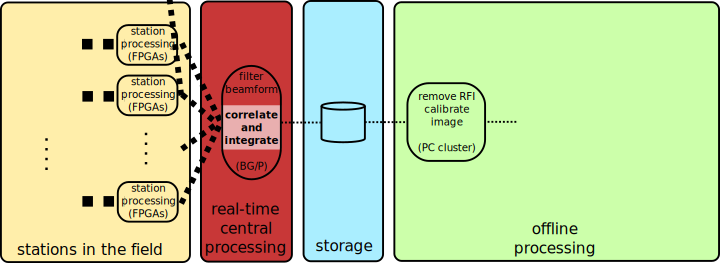
\includegraphics[width=\textwidth]{lofar-overview.pdf}
\caption{A simplified overview of the LOFAR processing.}
\label{fig:lofar-overview}
\end{figure*}

A global overview of the LOFAR instrument is given in
Figure~\ref{fig:lofar-overview}. LOFAR uses two different types of
antennas, the LBAs (Low-Band Antennas) and HBAs (High-Band Antennas).
The leftmost picture in the figure shows the low-band
antennas in the field.  Each LBA consists of one dipole per polarization,
while each HBA is organized as a tile, wherein 16 antenna elements are
combined. All antennas are dual polarized.

LOFAR's antennas are structured in a hierarchical way to limit the
costs of data transport and processing. Thousands of antennas are
necessary to obtain sufficient sensitivity. The antennas are
distributed over a large area to achieve a high angular resolution.
However, combining the data of all individual antennas centrally would
require too much network bandwidth and would result in excessive
computational requirements. Therefore, multiple antennas are grouped
to form a \emph{station}. Within a station, the information of all
individual antennas is weighted and summed.

Geographically, LOFAR consists of a compact core area and a number of
remote stations.  The heart of LOFAR will be installed in the Northern
part of the Netherlands.  The stations are distributed along 5
log-spiral arms with a diameter of approximately 360 km. The station
fields are centrally condensed, following a logarithmic distribution.
About 50\% of the stations are located in the central core. This inner
area can be operated for dedicated experiments with more data per
station.  Since other European institutes also show interest and are
building LOFAR stations, the maximal distance between LOFAR stations will be
extended, possibly to 1000 km.  In the past several years we have
deployed a number of prototype antennas, while the roll-out of
the real stations currently is in progress.

In total, XXX LBAs and YYY HBAs will be installed in a station. Each
station also features a cabinet where initial processing is done using
FPGAs.  Typical operations that are performed here include
analog-to-digital conversion, filtering and frequency selection. Also,
the signal is split into a number of different frequency ranges,
called \emph{subbands}.

All station data is transported to the central processing location in
Groningen via a wide area network (WAN), which uses owned and leased
light paths. We use UDP for data transport, since we can tolerate some
data loss. We do not use a reliable protocol such as TCP, because the
overhead would be to high for our purposes, and retransmissions in the
case of data loss would interfere with our real time requirements.

The UDP packets contain samples, where a sample is a complex number
that represents the amplitude and phase of a signal at a particular
time.  LOFAR supports $2\times4$, $2\times8$, and $2\times16$-bit
samples. Sampled data can be invalid for various reasons, such as
Radio Frequency Interference (RFI) and lost network packets.
Throughout the entire processing chain, we maintain which
data is marked as invalid, so that eventual images are not blurred by
bad data.  

The central processing is the main focus of this paper, and is done in
real time by an IBM Blue Gene/P supercomputer. We filter the data, and
split the subbands in narrower frequency bands called \emph{channels}, which allow
for more accurate RFI removal.
In addition, we perform phase shift and bandpass
corrections.  Finally, the signals from all stations are beamformed,
correlated and forwarded to a storage cluster, where results can be
kept for several days.  We will explain the central processing steps
in more detail in Section~\ref{sec:signal-processing}.

After the correlated data has been stored, further processing is done
\emph{offline}, on commodity cluster hardware. 
The results are calibrated for instrumental and environmental
effects, and known sources in the sky are subtracted to
enhance the dynamic range~\cite{Nijboer:07}. Finally, RFI is removed, 
and the correlation products are
transformed into an image.  The offline steps are done on
off-the-shelf cluster hardware, and are not part of the real-time
processing system described in this paper.


\section{The Blue Gene/P}

Initially, LOFAR used a 6-rack IBM Blue Gene/L supercomputer for real-time
processing of the station data.
We recently replaced the system by an equally powerful 2.5-rack Blue Gene/P.
%The consequences of this upgrade are described in Section~\ref{sec:upgrade}.
Below, we describe the key features of the Blue Gene/P.
More information can be found elsewhere~\cite{IBM:08}.

Our system contains 10,880 processor cores that provide 37.0~TFLOPS peak
processing power.
The system is built using SoC (System-on-a-Chip) technology that integrates
all processing and networking functionality on a single die.
One chip contains four PowerPC~450 cores, running at a modest 850~MHz clock
speed to reduce power consumption and increase package density.
Each core has two Floating-Point Units that provide support for
operations on complex numbers.
A core can sustain two fused multiply-adds per cycle.
The four cores share 2~GiB of main memory.
Although a node can run in \emph{SMP mode}, we run the application in
\emph{virtual node mode}, where the processor and memory of a node are split
into four independent, virtual machines.
This simplifies programming, since this allows single-threaded processing
on the compute cores.  % TODO: tree is shared resource; mention?
The compute nodes run a fast, simple, single-process kernel
\emph{(Compute Node Kernel, CNK)},

The Blue Gene/P contains several networks.
A fast \emph{3-dimensional torus\/} connects all compute nodes and is used
for point-to-point and all-to-all communications.
The \emph{collective network\/} is used for MPI collective operations,
but also for external communication.
A \emph{global interrupt network\/} provides support for fast barriers.
Additional networks exist for initialization, diagnostics, and debugging.

\begin{figure}[ht]
\begin{center}
\includegraphics[width=9cm]{pset.pdf}
\end{center}
\caption{A pset.}
\label{fig:pset}
\end{figure}

Each compute node is connected to an I/O~node via the collective network
(see Figure~\ref{fig:pset}).
An I/O~node uses the same hardware as a compute node, but has its Ethernet
interface connected and runs another operating system (a modified Linux kernel).
Since our application demands high bandwidths, our system is configured with
the maximum number of 1~I/O~node per 16~compute nodes (64~cores).
The group of one I/O~node and the compute nodes that are connected to it,
is called a \emph{pset}.
Our system has 160~psets in total, 64 per rack.
Normally, the I/O~node is used as a black box that provides transparent
communication from the compute nodes to external systems: all I/O-related
system calls on the compute nodes are forwarded to a daemon program that runs
on the I/O~node and performs the real operation.
In Section~\ref{sec:I/O-node-processing}, we show that it is much more
efficient to run part of the application software on the I/O~node.


\section{LOFAR Processing}

\begin{figure*}[ht]
\center{
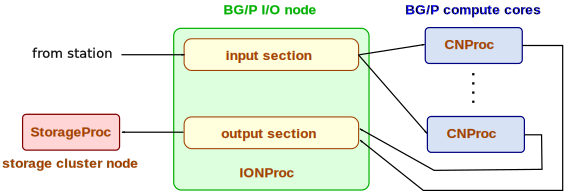
\includegraphics[width=0.8\textwidth]{processing-overview.pdf}
}
\caption{Simplified data flow diagram for the central processing pipeline.}
\label{fig:processing}
\end{figure*}

The LOFAR station data are centrally processed in real time by a collection
of three distributed applications.
These applications run on different platforms:
the Blue Gene/P \emph{I/O nodes}, the Blue Gene/P \emph{compute nodes}, and on
external (PC-like) \emph{storage nodes}.
Figure~\ref{fig:processing} shows how the data flows through the entire
processing chain.
The first application, \emph{IONProc}, runs on the Blue Gene/P I/O nodes.
Its main tasks are to receive the station UDP data, to buffer the data
for up to 2.5~seconds, and to forward it to the compute nodes.
The second application called \emph{CNProc}, runs on the Blue Gene/P compute nodes, where the
compute-intensive processing takes place.
The main tasks are to reorder the data across the compute nodes over the
internal torus network, to filter the data, and to correlate or beamform
the filtered data.
The resulting data are then sent back to the I/O-node application, that
collects the data from the compute nodes and
sends the data to the storage nodes.
This is where the third application (StorageProc) runs.
The storage nodes are PC-like systems with large disks.
The storage application collects the data from the I/O~nodes and writes the
data in an astronomical data format (AIPS++ Measurement Sets) to disk.


\section{I/O-node processing}
\label{sec:I/O-node-processing}

\begin{figure*}[t]
\center{
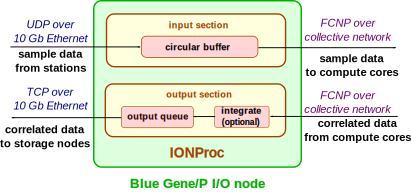
\includegraphics[width=0.8\textwidth]{ION-processing.pdf}
}
\caption{Simplified data flow diagram for the I/O nodes.}
\label{fig:ion-processing}
\end{figure*}

We use the Blue Gene in an innovative way, by running application software
on the I/O~nodes.
On the Blue Gene/L, this required rewriting major parts of the system
software~\cite{Iskra:08}, but this idea is much better supported on the
Blue Gene/P.

We run one multi-threaded process on each I/O~node that takes care of two
tasks: the handling of input and the handling of output.
The input section deals with UDP receipt of station data, and buffering and forwarding to the compute nodes.
The output section handles outgoing result data from the compute nodes, and forwards it to storage.
An I/O node may run both sections, either of them, or none at all, depending
on the configuration.
Both tasks are shown in Figure~\ref{fig:ion-processing}, and described in detail below.


\subsection{Input handling}
\label{sec:input-handling}

The FPGAs at a LOFAR station send UDP packets with sampled data over a
dedicated Wide-Area Network to a BG/P I/O~node.
To simplify the implementation, there is a one-to-one mapping between
stations and I/O~nodes, so that one I/O~node receives all data from a single
station.
However, handling the full 3.1~Gb/s data rate of a station on a relatively
slow CPU is quite a challenge.
Note that an I/O~node does not run the input section task if it is not
connected to a station.

The input section receives the UDP packets, taking care of out-of-order,
duplicated, and lost packets.
Each station uses four FPGAs to send data to its associated I/O~node,
each FPGA to a different UDP port.
The I/O~node runs four ``input'' threads, one thread per socket.
Multiple threads are necessary, since a single core is too slow to receive all
data.
Together, the threads receive a total of 48,828~packets per second.

The received UDP packets containing the samples are copied into a cicular buffer that holds the most recent
2.5~seconds of data.
The buffer serves three purposes.
First, it is used to synchronize the stations, since the travel times over
the WAN are higher for the remote stations than for the central stations.
Second, the buffer prevents data loss due to small variations in processing
times of the remainder of the pipeline.
Third, the buffer is used to artificially delay the stream of samples,
as we will explain in Section~\ref{sec:signal-processing}.
The buffer is limited by the small memory size, but due to good real-time
behavior of the application, 2.5~seconds is sufficient.

Another thread reads data from the circular buffer and sends the data to
the compute nodes for further processing.
It sends data in large bursts that contain approximately one second of samples.
Unfortunately, existing network software did not provide sufficient bandwidth
and consumed too much CPU time.
We therefore developed \emph{FCNP (Fast Collective-Network Protocol)}, a 
network library for high-bandwidth communication between the I/O~nodes and the
compute nodes~\cite{Romein:09a}.
FCNP, in contrast, achieves link-speed bandwidths for large messages, due to
its low overhead.
The data are sent directly from the circular buffer without additional copying.

When processing in real time, the NTP-synchronized wall-clock time
is used to trigger the sending of a new block of data.
A block of data containing samples from time $t_1$ to $t_2$ are sent some hundreds
of milliseconds (the WAN delay plus a safe margin) after $t_2$, whether or
not all data were factually received from the station.
This ruthless method assures real-time continuation of the correlator and
provides fault-tolerance against a failing station or WAN link.
In practice, this method does not cause any data loss.
An alternative mode processes pre-recorded data off-line and is frequently used
for experimental observations.
In this case, the input is \emph{reliably} read from file or TCP socket rather than
UDP.
In off-line mode we do not use the wall-clock time as
trigger, but we synchronize the threads that read and write the circular
buffer differently to prevent them from overrunning each other.


\subsection{Output handling}

The bulk of the signal processing is done on the compute nodes, on which we
elaborate in the next section.
The resulting output data are sent back to the I/O~node.
The second major task of the I/O-node application is to handle the output data.
This task performs four operations.

First, the data are received from the compute nodes, also using FCNP.
Second, the data are optionally added to previously received data from other
compute nodes in the pset, if integration over multiple seconds is desired.
Third, the (possibly integrated) output is queued in a buffer.
Fourth, another thread asynchronously dequeues the data and sends them to
a storage node, using a (reliable) TCP connection.

The queue improves real-time behavior and increases fault tolerance, since
it handles data on a best-effort basis.
If, for any reason, the data are not sent quickly enough to the storage node
(e.g., due to a disk or network failure), the queue fills up and subsequent
data are simply discarded until space is available.
This mechanism is important to keep the correlator running in real
time: it is much better to lose a small part of the data than to stall the
entire correlator and lose \emph{all\/} data.
In practice, under normal circumstances, no data are lost.


\subsection{Optimizations}

Processing power on the I/O~nodes is a scarce resource, and most observation
modes are I/O bound.
We performed many optimizations to improve processing speed.
An important improvement was to implement the function that copies data from a
received UDP packet to the circular buffer in assembly.
This way, we can exploit the efficient 16-byte load and
store instructions, which are unknown to the C++ compiler.
Unfortunately, the copy itself cannot be avoided, since an UDP packet contains
data of many frequency subbands that must be stored to different memory
locations.

Despite this optimization, we initially found that copying was very slow.
This was caused by the fact that the PowerPC~450 cannot handle
TLB\footnote{Translation Look-aside Buffer: a cache that caches
virtual-to-physical address mappings --- indispensable for efficient virtual
memory.} misses in hardware, but generates an interrupt and handles the fault
in software.
This is not a problem on the compute nodes, where the compute-node kernels 
map all memory using a few large pages, so that TLB misses do not occur.
However, the I/O~nodes run a Linux kernel that typically uses a page size of
4~KB, potentially generating a huge number of TLB-miss interrupts.

To avoid the interrupts, we use a modified ZeptoOS (Linux-based)
kernel\cite{Kazutomo:09}.
It allows a process to map 1.5~GiB (out of 2~GiB) of physical memory in its
virtual memory map, using six fixed mappings of 256~MiB that are never evicted
from the TLB.
Hence, this memory does not generate TLB misses.
The remainder of the memory is used for normal, paged operation.
The application uses this fast memory for the circular buffer and for the
output queues.
Copying data from received UDP packets to the input buffer is up to five times
faster than using paged memory.

To achieve good real-time behavior, we found that it is of utmost importance
to carefully manage thread priorities using the Linux real-time scheduler.
Since the compute nodes must always be able to proceed, they must be fed with
data without delays.
Therefore, the thread that sends data from the circular buffer to the
compute nodes runs at the highest priority, and is scheduled as soon as the
wall-clock time triggers.
The thread that reads results from the compute nodes is almost equally
important, since compute nodes will not accept new work before the previous
results were read by the I/O~node.
Other threads, such as the threads that read UDP data, and the threads that
send data from the output queues are also important, but if they would ever
fail to meet a real-time deadline, only a small amount of data is lost.
In practice, under normal circumstances, this rarely happens
(see Section~\ref{sec:ION-performance}).

%\begin{figure}
%\includegraphics[width=\columnwidth]{ion-performance.pdf}
%\caption{Performance breakdown of I/O-node processing.  See text.}
%\label{fig:ion-performance}
%\end{figure}



\section{Compute-node processing}

\begin{figure*}[t]
\center{
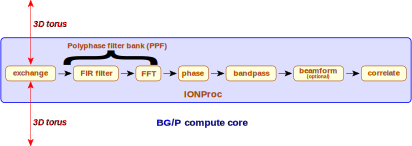
\includegraphics[width=0.8\textwidth]{CN-processing.pdf}
}
\caption{Simplified data flow diagram for the compute nodes.}
\label{fig:cn-processing}
\end{figure*}

The bulk of the signal-processing computations take place at the compute nodes.
In this section, we continue describing the processing pipeline depicted in
Figure~\ref{fig:processing}.
We explain how the data flow to the compute nodes, how the data are exchanged
between other compute nodes, what signal processing takes place, and which
optimizations we implemented.


\subsection{Scheduling}

\begin{figure}
\begin{minipage}[b]{9cm}
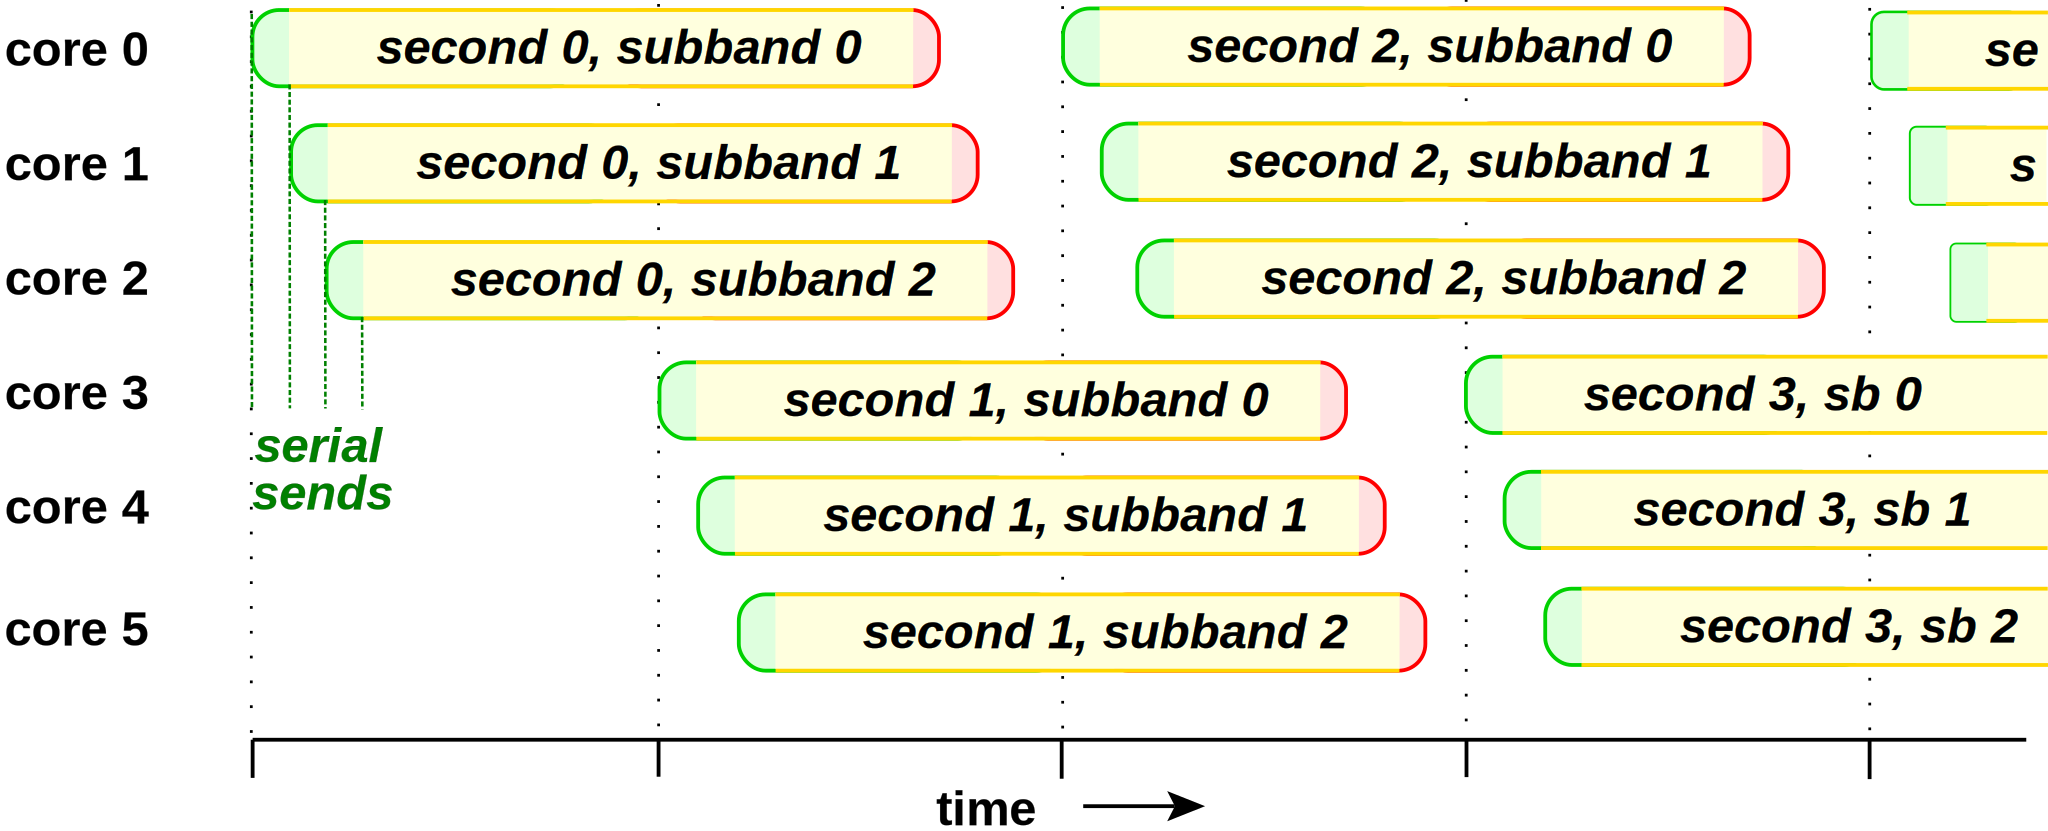
\includegraphics[width=9cm]{round-robin.pdf}
\caption{Round robin processing of work over compute-node cores.}
\label{fig:round-robin}
\end{minipage}
\hfill
\begin{minipage}[b]{5cm}
\includegraphics[width=5cm]{delay.pdf}
\caption{The left antenna receives the wave later.}
\label{fig:delay}
\end{minipage}
\end{figure}

The I/O~node chops the data stream that comes from the station into chunks of
one frequency subband and approximately one second of time.
Such a chunk is the unit of data that is sent to the compute node for further
processing.
Since processing a chunk typically takes much longer than one second,
the chunks are round-robin distributed over a group of processor cores,
as illustrated by Figure~\ref{fig:round-robin}.
Subsequent chunks are processed by different processor cores.
A core must finish its work before it is time to process the next chunk.
A core first receives data from the I/O~node (green in the figure),
processes them (yellow), sends back the results (red), and idles until the
I/O~node sends new data.

For simplicity, Figure~\ref{fig:round-robin} shows the processing of
three subbands on six cores.
In reality, scheduling is more complex.
First, the subbands that must be processed are (more or less) evenly divided
over the psets.
Typically, a pset is responsible for a fixed set of four to sixteen subbands.
Then, the subbands are round-robin scheduled over the 64~cores within the
pset.
For example, if a pset processes six subbands, every second, the next six
cores are scheduled and each of the cores will process one subband.
In this case, the available time to process one subband is ten seconds.
Since consecutive chunks of a particular subband are always processed by cores
within the same pset, the output for the subband is always sent via the same
I/O~node.
This greatly simplifies communication to the storage nodes and avoids
all-to-all communication over the 10~GbE switches.
If we would have scheduled all subbands over one large pool of compute cores
rather than psets, additional communication over the torus to reroute the
output would have been necessary.
On the Blue Gene/L, this could not be implemented efficiently due to the
inability to asynchronously communicate data using a DMA engine; on the
Blue Gene/P, it unnecessarily increases torus communication.


\subsection{All-to-All data exchange}

The compute nodes perform a large number of operations on the data, as shown in
Figure~\ref{fig:processing}.
The very first step is to exchange data with another group of processor cores.
This is necessary, because an I/O~node receives all frequency subbands from one
station, but the correlator requires one frequency subband from all
stations (we explain this in more detail below).
The data exchange is challenging, since it involves hundreds of gigabits per
second.
Unfortunately, an I/O~node cannot send the data directly from the circular
buffer to the compute core that will process the data, since the I/O~node is
only connected to the compute nodes in its own pset.
The data are thus first sent over the collective network from the I/O~node to
a compute node and then over the 3-D~torus network.
We use the 3-D~torus because of its high bandwidth and switching capabilities.

\begin{figure}
\begin{center}
\includegraphics[width=25mm]{colinear.pdf}
\end{center}
\caption{The bandwidth between colinear nodes is lower than on non-colinear nodes.}
\label{fig:colinear}
\end{figure}

The torus bandwidth between colinear and coplanar nodes is lower than between
non-coplanar nodes, since non-coplanar nodes communicate over more links
(in three dimensions) simultaneously.
Figure~\ref{fig:colinear} illustrates this; the bandwidth between nodes
\textsf{A} and \textsf{B} is (in theory) three times as high as the bandwidth
between nodes \textsf{A} and \textsf{C} (in practice, it is somewhat less).
Therefore, we schedule work that needs exchange of data 
on non-coplanar cores as much as possible.
We also avoid situations where multiple cores of the same processor need to
access the torus or collective network simultaneously, since these resources
are shared and simultaneous access decreases performance.
The program parts that implement the data exchange and scheduling are, in the
presence of many stations, many subbands, time slicing, round-robin core
allocation, and avoidance of resource conflicts, \emph{extremely\/}
complicated, but highly efficient.

% TODO alw we het hier over de BG/L gaan hebben, dan moeten we ergens (in de into?)
% de geschiedenis van LOFAR tot nu toe uitleggen. --Rob
On the BG/L, the data exchange was implemented synchronously, using
\texttt{MPI\_Alltoallv()}.
The BG/P, in contrast, uses DMA for the torus, allowing asynchronous
communication.
We re-implemented the data exchange using asynchronous point-to-point
communication, that overlaps the communication over the torus network with 
the data transfer from the I/O nodes to the compute nodes, and with
the next four processing steps.
As soon as a chunk of data from one station has arrived, the core starts
processing them, up to the point that the data from \emph{all\/} stations
are required.


\subsection{Signal Processing}
\label{sec:signal-processing}

After the data exchange, a core possesses the samples of one subband, from all
stations.
The data are processed through a number of filters, as briefly described below.
More details on the filters (except bandpass correction and beam forming)
can be found elsewhere~\cite{Romein:06}.

The subband data are first filtered by a \emph{Poly-Phase Filter bank\/} (PPF) that
splits a frequency subband into narrow frequency channels, trading time
resolution for frequency resolution.
The high frequency resolution allows for removal of narrow-band
\emph{Radio Frequency Interference\/} (RFI, e.g., caused by TV transmitters)
later in the pipeline.
Typically, a 195~KHz subband is split into 256~channels of 763~Hz, but the
filter supports any power-of-two number of channels.

As a side effect, the PPF implicitly converts 16-bit little-endian integer
samples to 32-bit big-endian floating point numbers, since the Blue Gene is
much better at floating-point processing than integer processing.
Since this conversion doubles the data size, the PPF runs \emph{after\/} the
data exchange.
The PPF itself consists of a number of 16-tap Finite Impulse Response (FIR)
filters, of which the outputs are Fourier Transformed.
The FIR filters and a 256-point FFT are implemented in assembly, for optimal
performance.
For other FFT sizes, we use the Blue Gene ``Vienna'' version of
FFTW~\cite{Lorenz:05}.

%The next step is to artificially ``delay'' the stream of station samples,
%to compensate for the fact that a celestial wave hits stations at different
%times~\cite[Sec.~2.1]{Romein:06}.

The next step is \emph{delay compensation}.
Due to the finite speed of light, the wave from a celestial source hits
stations at different times (see Figure~\ref{fig:delay}).
The time difference depends on the observation direction and the
station positions, and is continuously altered by the rotation of the earth.
Before the signals can be correlated, all station streams are aligned,
by artificially delaying the stream of station samples.
For example, a delay of 22\us can be achieved by shifting four 5.12\us
samples.
This shift was already done on the I/O~node, by moving the read pointer
of the circular buffer (see Section~\ref{sec:input-handling}).
Here, on the compute nodes, the remaining error (1.52\us) is corrected by
rotating the phase of the signal.
The phase rotation itself costs a complex multiplication per sample.
Since the rotation depends on the frequency, the correction is done after 
the PPF: the correction is more accurate on narrow frequency channels.
The delays are computed once per second and interpolated in frequency
and time for each individual sample.

The \emph{bandpass correction} step compensates for an artefact
introduced by a station filter bank (the PPF that creates the subbands).
Without correction, some channels contain more power than others.
The correction is performed by multiplying each complex sample by a real,
channel-dependent value that is computed in advance.
A station cannot correct for this artefact itself, since it is only visible
in channels, not in subbands.

The \emph{beam former} combines the data of all the stations by taking the
complex sum for each sample. As a result, the noise measured by the individual
stations level out, while any signals that were measured by multiple stations
are amplified. The output of the beam former is a single data stream,
representing a beam focused on a celestial source.

\subsection{Optimizations}

For optimal performance, most time-intensive code is written in assembly,
because the performance from compiled C++ code was by far not sufficient.
We maintain equivalent C++ reference code for testing and portability.
The assembly version hides load and instruction latencies, issues concurrent
floating point, integer, and load/store instructions,
and uses the L2 prefetch buffers in the most optimal way.
Most instructions are parallel fused multiply-adds, that sustain four
operations per cycle.

The assembly code minimizes the amount of memory loads by reusing a loaded
word as many times as possible.
The register file can hold 32~complex numbers \emph{TODO: cite many-core paper?}

Although the FIR filters, FFTs, delay compensation, and bandpass correction
are conceptually separate, consecutive blocks, their implementations are
highly interweaved to achieve better performance.
This avoids that four separate passes over all data are made.
Also, the data are laid out in memory in such a way that they are read
consecutively as much as possible, allowing burst transfers through the
cache hierarchy.
%This is not always possible, and in those cases we try to hide the memory
%Also, many of the computations are hidden by the memory access delays that
%are the result of a transpose in main memory.

%Although the correlator (including the other signal-processing steps) is a
%typical example of a streaming-data application, the perception ``byte goes
%in, byte comes out'' is misleading.
%The data are necessarily cut into large chunks, and basically every processing
%step needs the data in another order than the previous step produced.
%This maps poorly to the memory subsystem, that is not optimized for
%non-consecutive memory accesses.
%We also found that the round-robin replacement algorithm of the L1 caches
%XXX





%\section{I/O performance}

%The stations produce large amounts of data.
%The LOFAR specification requires 32~MHz of observation bandwidth with 16-bit,
%dual-polarized complex samples, yielding 2.1~Gb/s per station.
%However, both the station hardware and the Wide-Area network are capable of
%handling more data, up to 3.1~Gb/s per station.
%Also, some stations can be geographically split into two halves, doubling the
%data rate, but we treat both halves as separate stations, so that the number
%of stations increases but the data rate per station remains the same.

%As supercomputers are usually not optimized for external I/O, streaming data
%into the correlator at these rates is challenging.
%One of the reasons to choose for the Blue Gene as correlator was its atypical
%high number of external GbE interfaces, 768 in six racks.

%Despite its potential, streaming data into the machine at the required rates
%turned out to be problematic~\cite{Romein:06}.
%Each GbE interface has to sustain at least 550~Mb/s in and 200~Mb/s out
%(concurrently) to keep up with the stations.
%Initially, the total bandwidth (in and out) obtained in practice peaked at
%about 300~Mb/s.
%After a year of updating drivers and tuning parameters, aggregate bandwidths
%of about 850~Mb/s were seen, provided that four (out of sixteen) compute nodes
%communicated concurrently through the same I/O~node, effectively wasting
%3/16$^\mathrm{rm}$ of all compute resources.
%Also, the higher data rates were only seen using benchmark programs; the
%application exhibits more complex communication patterns that had a
%devastating impact on the performance.


%Although the BG/P is computationally very efficient,
%streaming the station data into the machine at the required data rates
%turned out to be a major problem in practice~\cite{Romein:06},
%despite the high number of I/O interfaces.
%For each 64~BG/P compute cores, there is one \emph{I/O~node\/} that
%has one external gigabit-Ethernet interface and transparently handles all I/O
%calls initiated by its associated compute cores through system call function
%forwarding (see Figure~\ref{fig:IOnode}).
%We found that the stock network system software was not particularly optimized
%for high-throughput I/O, and that the obtained bandwidths were insufficient
%for LOFAR operation.

%The dissatisfaction about the performance and about the I/O model in general
%led to a joint effort to redesign the entire network software infrastructure,
%and resulted in a new environment called {\em ZOID\/}~\cite{Iskra:08}.
%ZOID does not only yield better performance, but it is much more flexible,
%since it allows application code to be run on the I/O~node.
%With ZOID, we were able to move the receipt of the station data from the input
%cluster nodes to the BG/P I/O~nodes, so that the station data are sent
%directly through the WAN into the BG/P.
%Not having to build a separate input cluster results in an estimated cost
%saving of \euro700,000.




%\section{Upgrading from a BG/L to a BG/P}
%\label{sec:upgrade}
%
%Recently, the six-rack Blue Gene/L system was replaced by a 2.5-rack Blue
%Gene/P system, that provides approxiamately the same computational power.
%The biggest improvements of the BG/P over the BG/L are summarized below.
%First, the number of cores in a processor and the speeds of the processors and
%networks have increased.
%Second, the L1 caches are, unlike those of the BG/L, coherent.
%Third, the 3-D torus is extended with a DMA controller that allows
%asynchronous communication.
%Fourth, its programming environment has greatly improved; many System
%Programming Interfaces and part of the system software has become open source.
%Fifth, the 1-GbE technology of the BG/L was replaced by 10-GbE technology.
%Furthermore, there are improvements in reliability and power consumption.
%
%The improved programming environment and the change to 10-GbE technology
%had significant implications for our application.
%While the amount of FLOPS per rack has become 2.43 as high, the number of
%external interfaces has halved.
%As a consequence, each I/O~node has to handle (at least) four times as much
%data as on the BG/L.
%However, the total processing power on the BG/P has only improved by a factor
%of 2.43, while the load on the I/O~nodes of the BG/L was already problematic!
%Also, we measured that the link speed of the collective network that connects
%the I/O~node to the compute nodes cannot carry more than 6.54~Gb/s payload.
%%Taking the high costs of the UDP/IP protocol stack into account, we thought
%%that handling the full station data rate of 3.1~Gb % FIXME
%
%

% JD SCRATCHPAD
% -------------------
%\section{Flexibility}

%One of the main benefits of processing the telescope data in software rather than hardware is the increased flexibility of our setup.

%The LOFAR frequency range (10 -- 250 MHz) allows the observation of many interesting astronomical phenomena. 

%Apart from the imaging pipeline which we described so far, we have implemented several pulsar pipelines, and plan to implement the Epoch-of-Reionization pipeline.

% silicon vs software / asm vs C
% multiple pipelines: pulsars, eor (note: maintain order in intro)
%	- component overlap / synergy
%	- reuse of expensive asm
%	- flexible C:
%		+ fast implementation
%		+ early feasibility and accuracy testing
%		- slower => less throughput, but sometimes
%			+ runtime not significant
%			+ subsequent processing too expensive anyway,
%			  so we have the time
% pulsar pipeline:
%	- experimental phase, C implementation
%	- used to detect pulsars
%	- pulsars useful for clock calibration
%	- fast implementation due to reuse and C
%	- lofar is experimental. astronomers need to learn possibilities.
%	  C allows quick change in functionality
%
% eor (future work):
%	- first detectable objects in the universe (universe was opaque before that)
%	- due to redshift, wavelength of H is 1.5-3m (115-180MHz)
%	- 
\section{The output of the correlator}

\begin{figure}
\begin{center}
\includegraphics[width=12cm]{fringe.jpg}
\end{center}
\caption{Correlations from a 9-hour observation.  See the main text for
an explanation.}
\label{fig:fringe}
\end{figure}

A graphical representation of the correlator output is depicted in
Figure~\ref{fig:fringe}.
The figure shows the cross-correlations from two stations during a 9-hour
observation.
The horizontal axis varies in time;
the vertical axis represents the 256~channels of one frequency subband.
Each pixel corresponds to a (complex) correlation, where the color represents
the phase of the signal; the intensity matches the amplitude (power).
The phase changes over time, due to the earth rotation that alters the
relative position of the observed sources.
The white spots are caused by RFI; these bad data are detected and
ignored in the remainder of the processing pipeline.

The correlations are used to create images.
Even with the limited amount of prototype antennas that have been employed
during the last few years, impressive (all-sky) images were made.
Also, the prototype pulsar pipeline software successfully detected several
known pulsars.



\section{Performance}

Since only a small number of LOFAR stations has already been constructed
(the majority will become operational later this year), we will provide 
performance measurements with externally generated artificial data.
We use one Blue Gene/P rack to generate UDP data, another rack for the
correlator, and the remaining half rack to receive and dump the correlated
data.
The simulation is realistic, since the correlator runs exactly
the way it would run with real station data.
The storage section, however, does not write the data to disk, since we do
not have enough storage nodes available yet, but this does not influence the
performance measurements of the correlator.
With one rack, we can process up to 64~stations, one per I/O~node.

\begin{table}[ht]
\begin{center}
\begin{tabular}{|l|rrr|}
\hline
Observation mode	 & \textsf{A}	& \textsf{B}	& \textsf{C}	\\
\hline
nr.\ bits per sample	 & 16		& 8		& 4	\\
max.\ nr.\ of subbands	 & 248		& 496		& 992	\\
nr. channels per subband & 256		& 256		& 256	\\
max.\ nr.\ of stations	 & 64		& 64		& 48	\\
\hline
input bandwidth (nr.\ I/O nodes * Gb/s)  & 64 * 3.1  = \bf{198} & 64 * 3.1 = \bf{198} & 48 * 3.1 = \bf{149} \\
output bandwidth (nr.\ I/O nodes * Gb/s) & 62 * 0.58 = \bf{36}  & 62 * 1.2 = \bf{74}  & 62 * 1.3 = \bf{81} \\
\hline
available compute time per subband (s)	 & 16.1	     & 8.05     & 4.03     \\
\hline
\end{tabular}
\end{center}
\caption{Characteristics of three realistic, challenging observation modes.}
\label{tab:observation-characteristics}
\end{table}

We show the performance results of the application by means of three
challenging observation modes which are likely to be commonly used.
The characteristics of these modes are listed in
Table~\ref{tab:observation-characteristics}.
Mode~\textsf{A} is the standard mode, where the stations send 16-bit samples.
In this mode, the FPGAs can send at most 248~subbands.
The 248~subbands are evenly divided over 62~psets, so that each pset processes
4~subbands (the remaining two psets handle input data, but do not correlate).
Since there are 64~cores in one pset and an integration time equals 1.007~s (768 samples),
the available time to process one chunk of data (1 subband) is 16.1~s.

Mode~\textsf{B} trades accuracy for observation bandwidth, by reducing the
sample size to 8~bits and doubling the number of subbands.
This implies that the total input data rate remains the same, but that the
processing requirements and output data rate double.
The 62~psets that are used to correlate have to process 8~subbands each,
reducing the available time per subband to 8.05~s.

Mode~\textsf{C} uses 4-bit samples, and is only suitable for frequency
subbands that are mostly free of RFI (otherwise, the bits are used to encode
the RFI, not the signal of interest).
This mode is planned for \emph{Epoch-of-Reionization} observations, where the high number of subbands
is used to observe sky in six directions simultaneously.
If the same amount of stations were used, the processing requirements and
output data rate would double again, but EoR observations will only use the
stations near the center, not the remote ones.
The exact number of stations that must be correlated is not yet known, but is
likely between 36 and~46.
For the performance measurements, we assume the most challenging case, and use 48~stations.


\subsection{Computational performance on the I/O Nodes}
\label{sec:ION-performance}

\begin{figure}
\hspace{9mm}
\subfigure[As function of number of subbands.  The input samples are 8~bit,
  and in total, 64 stations are used.]{
  %\includegraphics[width=\columnwidth]{ion-performance.pdf}
  \makebox[92mm][l]{
  \includegraphics[width=13cm]{ion-performance.pdf}
  }
  \label{fig:ion-performance-func-subbands}
}
\hspace{1cm}
\subfigure[For various observation modes.]{
  \hspace{25mm}
  \label{fig:ion-performance-obs-mode}
}
\caption{I/O node performance breakdown.}
\label{fig:ion-performance}
\end{figure}

The I/O requirements are challenging, and the processing power on the I/O~nodes
is limited.
Figure~\ref{fig:ion-performance} shows where the processor cores of the
I/O~nodes spend their time in various situations.
A load of 100\% means that all four cores are fully occupied.
A load above 85\% must be avoided to prevent major data loss.

We first show how the performance scales with the number of subbands.
We again use a setting similar to observation mode~\textsf{B}, for up to
496~subbands, see Figure~\ref{fig:ion-performance-func-subbands}.
The I/O~nodes receive and forward the samples
of one station (up to 3.1~Gb/s) and send the correlations of up to 8~subbands
to storage (up to 1.2~Gb/s).
The figure shows that most time is spent in the receipt of UDP packets.
This amount is partially independent of the number of subbands, since a lower
number of subbands decreases the packet size (down from 7,998~bytes), but not
the amount of packets. The I/O nodes have to handle 48,828~packets per second in all cases.
All other work scales linearly with the amount of subbands.

Figure~\ref{fig:ion-performance-obs-mode} shows the performance breakdown
for the three challenging observation modes.
In the standard 16-bit sample mode, the stations can produce at most
248~subbands (obs. mode A).
Hence, the output data rate (the lower two bars) is twice as low as in the
8-bit mode of scenario B.
Also, copying 16-bit samples into the circular buffer is somewhat more
efficient, due to L3-cache effects.
In the 4-bit mode, the number of stations is computationally limited to
about~48, because of the high number of 992~subbands.
Due to the reduced number of stations, the output data rate is only 13\%~higher
than in the 64-station/8-bit mode.
%We initially thought that this mode would really require two racks, but are
%actually able to perform it on a single rack.

%The I/O node application is optimized so thoroughly that it can receive a
%station input of 3.1~Gb/s --- 51\% above the initial LOFAR requirements; the
%absolute maximum that a station can generate.
%Additionally, an I/O node sends up to 580~Mb/s to storage.
%Figure~\ref{fig:ionode-load} shows where an I/O~node spends its time.
%Even at these data rates, the idle time is 34\%, more than sufficient for
%smooth, real-time handling of data.

%The most time-consuming operation (36\%) is the receipt of UDP packets by
%the kernel, as each I/O~node receives 48,828~UDP packets of 7,998~bytes
%per second.
%Copying the received data to the circular buffer adds 7\% to the load.
%FCNP efficiently forwards the data directly from the circular buffer to the
%compute nodes~(15\%) and receives the correlated data from the compute
%nodes~(3\%).
%Sending the data to the storage nodes (over TCP) takes~5\%.
%Other tasks have negligible impact on the processor load.

Both FCNP and the fixed TLB mappings significantly contribute to the low
resource usage.
Without either of them, the application cannot handle these data rates in
real time.

The data loss due to missed UDP packets is low: only between 1 per $10^6$ and
1 per $10^4$ packets are dropped under full load.
These numbers include the data loss caused by the (software) generators and by
the 10~GbE network switches.
The data loss is negligible to other places where data can be lost,
(e.g., the flagger sometimes rejects tens of percents of the data due to RFI),
and does not hurt the astronomical signal quality.
With the I/O-related optimizations, we obtain bandwidths that are on a par
with the achieved processing data rates.
Unless the requirements change, sufficient bandwidth is obtained to support
all observation modes on a single rack.
If the need would arise to achieve even higher bandwidths, UDP packet receipt
could be optimized by not using the \texttt{read()} system call interface,
but by using another interface that reads the data directly from kernel buffers
and does not enforce a (370~MiB/s !) kernel-to-user-space copy.
Right now, we felt no need to implement the required kernel changes.
Alternatively, the second rack could be used.
%If future observation modes would require higher output data rates, we may
%optimize the memory copy routines in the Linux kernel by using the
%Blue-Gene-specific 16-byte load/store instructions, rather
%than standard 4-byte PowerPC load/stores.
%We think this will reduce the system time of I/O operations.


\subsection{Computational performance on the Compute Nodes}

\begin{figure}
\hspace{9mm}
\subfigure[Performance as a function of the number of stations.  The input samples are 8~bit,
  and in total, 496 subbands are processed.]{
  %\includegraphics[width=\columnwidth]{cn-performance.pdf}
  \makebox[92mm][l]{
  \includegraphics[width=13cm]{cn-performance.pdf}
  }
  \label{fig:cn-performance-func-stations}
}
\hspace{0.8cm}
\subfigure[Performance of three challenging observation modes.]{
  \hspace{25mm}
  \label{fig:cn-performance-obs-mode}
}
\caption{Compute node performance breakdown.}
\label{fig:cn-performance}
\end{figure}

Figure~\ref{fig:cn-performance} shows how the compute nodes spend their time.
The seven major tasks are each represented by a different color in the bar
graph; the size of each bar is proportional to the contribution to the total
work load.
The vertical axis shows the execution time to process one subband with
1.007~second of station samples.

Before comparing the performance of the three observation modes described
above, we show how the performance scales with the number of stations.
Figure~\ref{fig:cn-performance-func-stations} shows execution times for up to
64~stations in a setting that is similar to observation mode~\textsf{B}.
The $O(n^2)$ complexity of the correlator is clearly visible (the correlations
between all \emph{pairs\/} of stations are computed), while other
components scale linearly with the number of stations.
Despite the high data rates, I/O~requires hardly any time \emph{on the compute nodes}.
It is important to realize that the time for input or output cannot exceed $1/64^\mathrm{th}$
of the total time, since the associated I/O~node also needs time to communicate
with the other 63~cores in the pset.

%The \emph{available\/} runtime depends on the number of subbands that must be
%processed: with 496~subbands, most of the 64~psets process 8~subbands, and
%with 64~cores in one pset, there is 8.053~second to process one chunk of data.
%Doubling the number of subbands halves the available processing time, and in
%the 4-bit mode, up to about 50~stations can be supported on a single rack.

The performance results hardly differ for the 16-bit and 4-bit modes (not shown),
since only the performance of the the data receipt from the I/O~node and data
exchange phase are affected by the sample size, 
both of which hardly contribute to the total runtime.
This is clearly illustrated by Figure~\ref{fig:cn-performance-obs-mode},
where the execution times for observation modes \textsf{A} and \textsf{B}
are nearly the same.
The run time for observation mode \textsf{C} is lower, since this mode
processes 48 rather than 64~stations.
All modes run within their real-time constraints of 16.1, 8.05, and 4.03
seconds respectively.
The load on the compute nodes is 35\%, 70\%, and 84\% repectively.

@@@ TODO: hoeveel sneller is de FFT in tijd? --Rob @@@
The correlator is extremely efficient: it achieves 96\% of the FPU peak
performance, thanks to the highly-optimized assembly code.
The FIR filter runs at 86\% of the peak performance, and the hand-crafted
256-point FFT run at 44\%%
\footnote{The FFT requires 8,390~operations, 18\% less than an unoptimized
$5n \log_2 n$ implementation.  Although an unoptimized FFT could achieve even
more than 44\% FPU efficiency, its absolute run time would be higher.}
(``Vienna'' FFTW achieves 34\%, which is also high for a FFT).
Compared to equivalent C++ code that is written for clarity and not
specifically tuned for optimal performance, the hand-written assembly code is
typically an order of magnitude faster.

Due to all optimizations, the correlator can process 50\% more data than
the specifications require, on only half the amount of planned resources.
Only if the need to correlate more than 64~stations would ever arise, or if
significant additional real-time signal processing would be needed, the
second rack must be employed.


\section{Related Work}

%LOFAR is not the only radio telescope of which the data are processed in software. In fact,
%in the 1960s, several observatories~\cite{Bare:67,Moran:67} recorded their input on high-speed tapes
%and processed it on IBM 360 mainframes. However, as the volume of the data increased, the mainframes were no longer capable of processing the data in an acceptable amount of time, and custom hardware had to be used instead.

%Due to the massive increase in processing power since the 1960s, software processing of telescope
%data is once again feasible. Several efforts to do so have been started. However, to the best of our knowledge,
%LOFAR is the only system capable of processing high data rates from a large number of stations at
%real time.

The idea of implementing a correlator in software has been adopted by others as
well.
However, the LOFAR correlator is the only system capable of processing a large
number of inputs at high data rates in real time.
Other systems handle only a few inputs, handle limited data rates, or do not
run in real time.

Deller et al.~\cite{Deller:07} have developed the DiFX distributed
software correlator, which is to be deployed on a cluster of PCs.
Due to the use of commodity hardware, both their communication and
computational capabilities are substantially lower than those available in
our BlueGene/P.
%As a result, they cannot handle the width and number of input streams that we
%process in LOFAR.
The real-time data processing of the Murchison Widefield Array (MWA) telescope
is implemented partially in software.
However, their correlator, computationally the most demanding part of the
processing pipeline, is not implemented in software, but on an
FPGA~\cite{Ord:08}.
Finally, the Joint Institute for VLBI in Europe (JIVE) develops a new software
correlator for e-VLBI observations, but is not capable of processing telescope
data in real time \textbf{JD: check}.

In another paper, we compare the efficiency of five different many-core
architectures (GPUs from Nvidia and ATI, the IBM Cell BE, the Blue Gene/P,
and the Intel Core~i7) for correlation purposes~\cite{Nieuwpoort:09}.


\section{Conclusions and future work}

We have shown that telescope data can be processed in real time using software, even if the
input data rate is hundreds of gigabits per second. In fact, our LOFAR processing software was
efficient enough to exceed the LOFAR specifications by 50\%. We use several parts of our BlueGene/P
supercomputer in unconventional ways in order to achieve high performance. The I/O nodes were meant
to be merely a bridge between the compute nodes and the outside world, but we equip them
with custom software in order to deal with the 3.1 Gb/s input, the output, and to perform both
pre- and post-processing. Also, we use a custom network protocol called FCNP to be
obtain the required data rates to and from the compute nodes.

Our implementation benefits from a mix of C++ and assembly. The C++ code base offers the flexibility
to implement several pipelines and to easily combine and reuse components. The use of assembly allows
the performance critical parts to run at high efficiency. For example, our correlator, one of the core
components we describe in this paper, runs at 96\% of the FPU peak performance.

% Conclusions:
%	- telescope data can be processed in real time using software
%	- exceed specs by 50%
%	- flexibility and speed through the mix of C and assembly
%	- core component is correlator, running at 96% of FPU peak performance
%	- unconventional use of I/O node and network stack pays off

The flexibility of our setup allows more pipelines to be implemented in order to facilitate several
modes of observation. We plan to finish the implementation of several pipelines, for the detection
and analysis of pulsars, but most notably to obtain images from the End-of-Reionization era. Furthermore,
we plan to extend our on-line processing, for example by including RFI detection and on-line calibration.

% Future work: RFI, online calibration, other pipelines


\section*{Acknowledgments}

\textbf{Rob: AstroStream ack}.
We thank Ger van Diepen, Martin Gels, Marcel Loose and Ruud Overeem
for their contributions to the LOFAR software.
We also thank Kamil Iskra and Kazutomo Yoshii from Argonne National Laboratory
for their work on ZOID and ZeptoOS.
Todd Inglet, Tom Liebsch, and Andrew Taufener from IBM Rochester provided the
necessary support to optimally use the Blue Gene/P.

LOFAR is funded by the Dutch government in the BSIK programme for
interdisciplinary research for improvements of the knowledge infrastructure.
Additional funding is provided by the European Union, European Regional
Development Fund (EFRO) and by the ``Samenwerkingsverband Noord-Nederland,''
EZ/KOMPAS.

\bibliographystyle{plain}
\bibliography{lofar}

\end{document}
